%%A program to make slides on pythagoras theorem
%to include themes, animation, title slide, blocks, table and figures

\documentclass[10pt]{beamer}
\usepackage{epstopdf}
\usepackage{url}			%for url's to be included in tex file 
\usepackage{hyperref}		%for url's to be included in pdf file
\usepackage{multirow}		%to be used in tables
\usepackage{graphicx}		%for graphics(here it is used to insert images)
\usepackage{wasysym}		%for using various symbols

\usetheme{Warsaw}
%default is there if not specified-default/Warsaw/Margaw/Madrid
\setbeamercovered{invisible}
%we can use transparent/invisible/dynamic too
\usecolortheme{beaver}
%color scheme is beaver
\setbeamertemplate{navigation symbols}{}
%remove navigation symbols

\title[Pythagoras theorem]{A Visual Proof Of The Pythagorean Theorem}
%Mine proof of pythagoras
\subtitle{Pythagoras theorem}
\author[Pythagoras of Samos]{Pythagoras}
%I am pythagoras
\date{\today}
%todays date


\AtBeginSection[]
{
	\begin{frame}<beamer>
		\transboxout
		\frametitle{Outline}
		\tableofcontents[currentsection]
	\end{frame}
}

\begin{document}
%\maketitle              %it will show the title page again
\begin{frame}
	\titlepage			%it will show the title page just like maketitle
\end{frame}

\begin{frame}{Outline}
	\transfade
	\tableofcontents
\end{frame}

\section{Introduction to Pythagoras Theorem}

\begin{frame}{Introduction}
\label{sec:intro}

%This is a introduction to my proof on pythagoras theorem  and its details....
\transdissolve
The theorem is of fundamental importance in Euclidean Geometry where it serves 
as a basis for the definition of distance between two points.
\emph{The area of the square built upon the hypotenuse of a right
triangle is equal to the sum of the areas of the squares upon the
remaining sides}.
\end{frame}

\section{Theorem, Definition And Relation}
\label{sec:def}
\subsection{Theorem}
\begin{frame}{Theorem}
\begin{block}{Pythagoras Theorem}
\transfade
The square of the hypotenuse (the side opposite the right angle) is equal to the sum of the squares of the other two sides
\end{block}
\end{frame}

\subsection{Definition}
\begin{frame}{Definition}
\transfade
The theorem that the sum of the squares of the lengths of the sides of a right triangle is equal to the square of the length of the hypotenuse.
\end{frame}

\subsection{Relation}
\begin{frame}{Relation}
\transfade
	\begin{itemize}
	\item In mathematics, the Pythagorean theorem or Pythagoras theorem is a relation in Euclidean geometry among the three sides of a right triangle.
	\pause
	\item The Pythagorean Theorem states that for a right triangle, the sum of the squares of the sides is equal to the square of the hypotenuse. 
	\pause
	\item Pythagoras Theorem can also be stated as the square formed on the hypotenuse of a right-angled triangle has the same area as the sum of the areas of the squares formed on the other two sides.
	\end{itemize}
 The theorem can be written as an equation relating the lengths of the sides a, b and c, often called the Pythagorean equation:
\begin{equation}
\label{one}
a^2+b^2=c^2
\end{equation}
where c represents the length of the hypotenuse, and a and b represent the lengths of the other two sides.
%\textcolor<2>{orange}{Example Text
\end{frame}

\section{Importance of Pythagoras theorem}
\label{sec:importance}
\subsection{Importance in Triangles}
\begin{frame}{Importance in Triangles}
\transfade
There are many uses for the Pythagorean Theorem, that is the main reason why it is important. You can use the Pythagorean Theorem to find out if a triangle is an acute triangle, obtuse triangle or a right triangle. If the Theorem works and the side lengths squared is equal to the hypotenuse squared, then it is a right triangle, if the hypotenuse squared is longer than the two side lengths squared and added together then the triangle is obtuse. If the hypotenuse squared is shorter than the two side lengths squared and added together then the triangle is acute.
\end{frame}
\subsection{Importance in Finding Missing Side Lengths}
\begin{frame}{Importance in Finding Missing Side Lengths}
\transfade
Another reason the Pythagorean Theorem is imported is it can help you find missing side lengths. Not only can it help you find the third side length to a right triangle, but it can also help you find the missing side lengths to squares and rectangles when the triangles are pushed together. The pythagorean Theorem can help build rectangles and squares.
\end{frame}

\section{Proof of the Pythagorean Theorem using Algebra}
\label{sec:proof}
\subsection{Figure}
\begin{frame}{Figure}
\begin{figure}[htb!]
  \begin{center}
    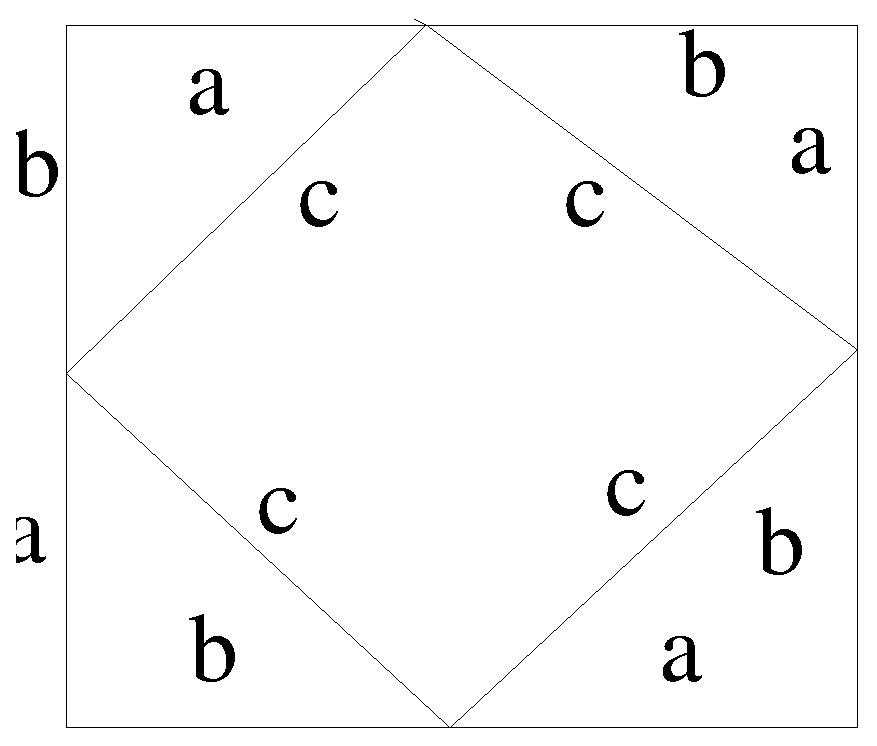
\includegraphics[width=40mm,scale=0.5 ]{fig9.eps}
   \end{center}
  \caption{Figure for pythagoras theorem}
  \label{image1}
\end{figure}
We can show that using Algebra.Take a look at the diagram above. It has that "abc" triangle in it (four of them actually).Figure~\ref{image1} shows a photo of a square contains various figures. We will calculate the areas of the respective figures in the below subsections.
\transfade
\end{frame}

\subsection{Area of Whole Square}
\label{a_square}
\begin{frame}{Area of The Square}
\begin{figure}[htb!]
  \begin{center}
    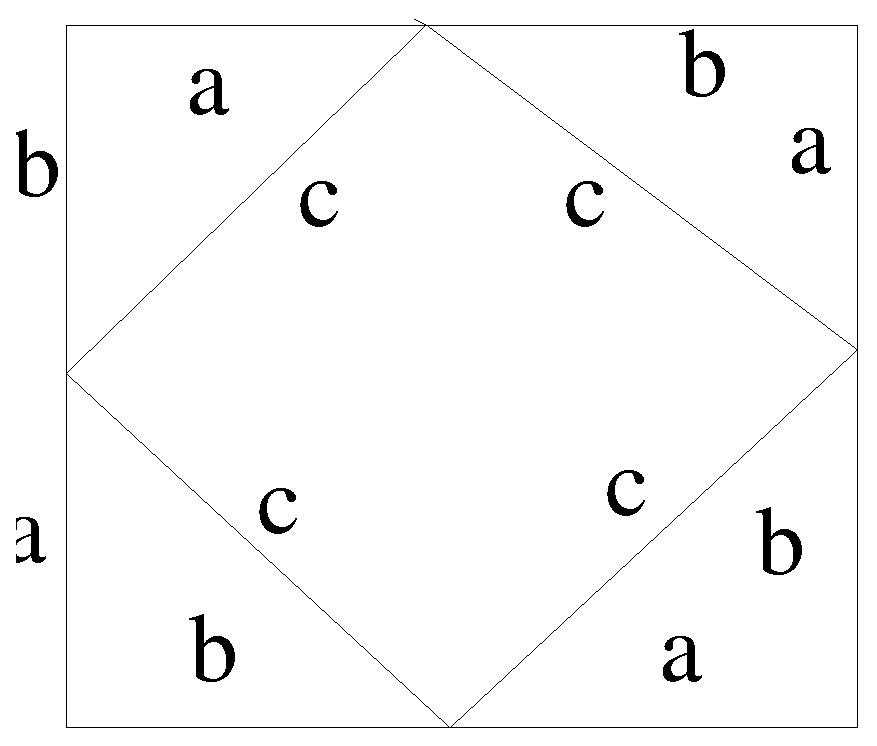
\includegraphics[width=25mm,scale=0.5 ]{fig9.eps}
   \end{center}
  \caption{Figure for pythagoras theorem}
  \label{image1}
\end{figure}
\transfade
It is a big square, with each side having a length of a+b, so the total area is:
$$A = (a+b)(a+b)$$
\end{frame}
\subsection{Area of Other Pieces}
\label{a_pieces}
\begin{frame}{Area of Other Pieces....(continue)}
\begin{figure}[htb!]
  \begin{center}
    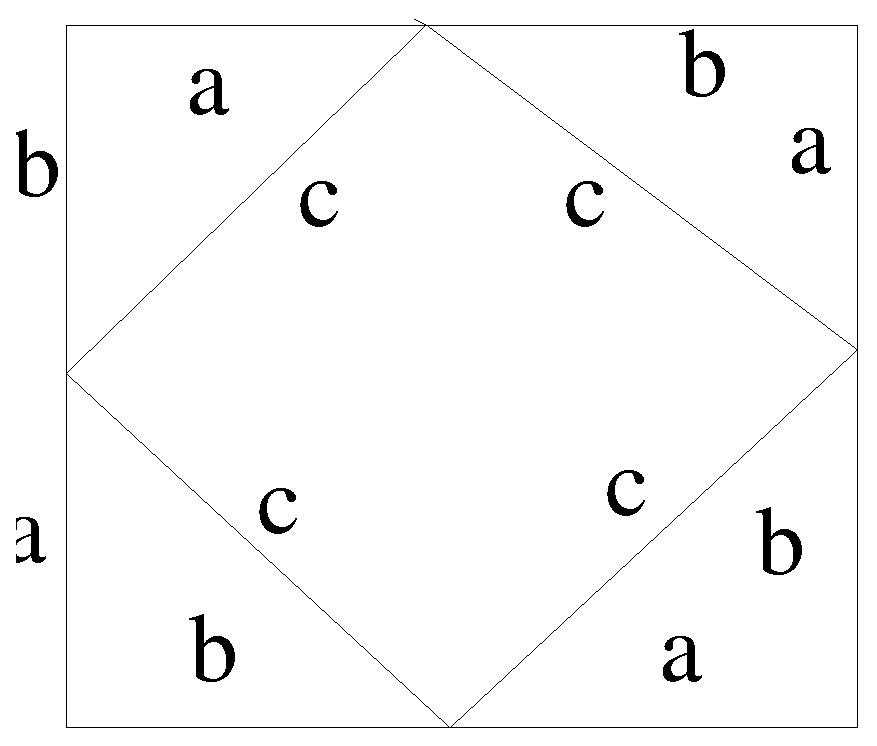
\includegraphics[width=25mm,scale=0.5 ]{fig9.eps}
   \end{center}
  \caption{Figure for pythagoras theorem}
  \label{image1}
\end{figure}
\transfade

Now let's add up the areas of all the smaller pieces:\newline
First, the smaller (tilted) square has an area of:
\begin{equation}
\label{two}
A = c^2 
\end{equation} 
And there are four triangles, each one has an area of 
\begin{equation}
\label{three}
A =\frac{1}{2} ab
\end{equation}
\end{frame}

\begin{frame}{Area of Other Pieces....(continue)}
\begin{figure}[htb!]
  \begin{center}
    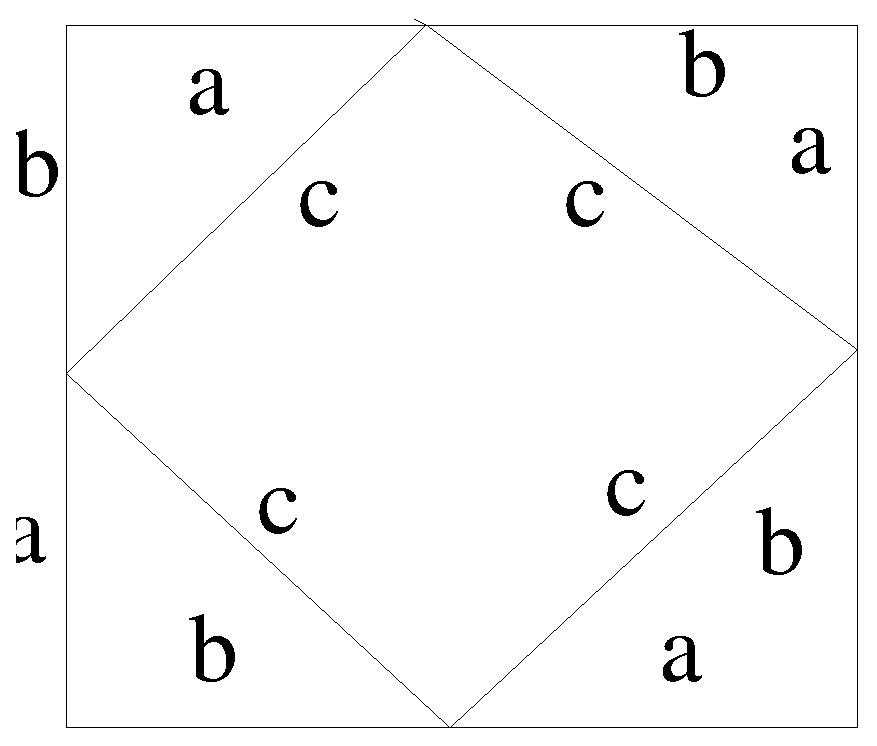
\includegraphics[width=25mm,scale=0.5 ]{fig9.eps}
   \end{center}
  \caption{Figure for pythagoras theorem}
  \label{image1}
\end{figure}

\transfade
So all four of them combined is	
\begin{equation}
\label{two}
A = 4(\frac{1}{2}ab) = 2ab
\end{equation} 
So, adding up the tilted square and the 4 triangles gives: 
\begin{equation}
\label{five}
A = c^2 +2ab
\end{equation}
\end{frame}

\subsection{Both Areas Must Be Equal}
\label{a_equal}
\begin{frame}{Both Areas Must Be Equal}
The area of the large square is equal to the area of the tilted square and the 4 triangles. This can be written as (from equation ~\ref{five}):\newline
\transfade
\begin{equation}
\label{six}
(a+b)(a+b) = c^2 +2ab
\end{equation}
Now, let us rearrange equation ~\ref{six} to see if we can get the pythagoras theorem:
\begin{equation}
\label{seven}
(a+b)(a+b)	=	c^2 + 2ab
\end{equation}
Expand (a+b)(a+b) in equation ~\ref{seven}:
\begin{equation}
\label{eight}
a² + 2ab + b²	=	c^2 + 2ab
\end{equation}
Subtract "2ab" from both sides in equation ~\ref{eight}:\newline	 
\centerline {$a^2$ + $b^2$	=	$c^2$}\newline

The following above statements gives us the proof of pythagoras theorem. Also, we can see the table below to see the correctness of theorem.
\end{frame}

\section{Examples and References of Pythagoras Theorem}
\subsection{Examples of Pythagoras theorem}
\begin{frame}{Examples of Pythagoras theorem}
\begin{exampleblock}{Few examples on Pythagoras theorem}
\begin{table}[bht]%\Large
	\begin{center}
		\begin{tabular}{c c c c c c c}
			\hline\hline
			Lenght a & Height b & Hypotenuse c & $a^2$ & $b^2$ & $c^2$ & $a^2$+$b^2$    \\
			\hline
			\hline
			4 & 3 & 5 & 16 & 9 & 25 & 25 \\
			8 & 15 & 17 & 64 & 225 & 289 & 289\\
			9 & 40 & 41 & 81 & 1600 & 1681 & 1681\\
			5 & 12 & 13 & 25 & 144 & 169 & 169 \\
			7 & 24 & 25 & 49 & 576 & 625 & 625\\
			\hline
		\end{tabular}
		\caption{Examples}
		\label{sec:examp}
	\end{center}
\end{table}
\end{exampleblock}
\transblindshorizontal
\end{frame}

\subsection{References(Books)}
\begin{frame}{References(Books)}
\nocite{*}
\bibliographystyle{plain}
\bibliography{b1}
\transfade
\end{frame}

\subsection{References(Links)}
\begin{frame}{References(Links)}
\begin{block}{Here are some links used to make this pdf:}
	\url{http://www.mathsisfun.com/geometry/pythagorean-theorem-proof.html}
	\url{http://en.wikibooks.org/wiki/LaTeX/Basics}
	\url{http://www.maths.tcd.ie/~dwilkins/LaTeXPrimer/}
\transfade
\end{block}
\end{frame}



\end{document}


